% Options for packages loaded elsewhere
\PassOptionsToPackage{unicode}{hyperref}
\PassOptionsToPackage{hyphens}{url}
%
\documentclass[
]{article}
\usepackage{amsmath,amssymb}
\usepackage{lmodern}
\usepackage{iftex}
\ifPDFTeX
  \usepackage[T1]{fontenc}
  \usepackage[utf8]{inputenc}
  \usepackage{textcomp} % provide euro and other symbols
\else % if luatex or xetex
  \usepackage{unicode-math}
  \defaultfontfeatures{Scale=MatchLowercase}
  \defaultfontfeatures[\rmfamily]{Ligatures=TeX,Scale=1}
\fi
% Use upquote if available, for straight quotes in verbatim environments
\IfFileExists{upquote.sty}{\usepackage{upquote}}{}
\IfFileExists{microtype.sty}{% use microtype if available
  \usepackage[]{microtype}
  \UseMicrotypeSet[protrusion]{basicmath} % disable protrusion for tt fonts
}{}
\makeatletter
\@ifundefined{KOMAClassName}{% if non-KOMA class
  \IfFileExists{parskip.sty}{%
    \usepackage{parskip}
  }{% else
    \setlength{\parindent}{0pt}
    \setlength{\parskip}{6pt plus 2pt minus 1pt}}
}{% if KOMA class
  \KOMAoptions{parskip=half}}
\makeatother
\usepackage{xcolor}
\usepackage[margin=1in]{geometry}
\usepackage{color}
\usepackage{fancyvrb}
\newcommand{\VerbBar}{|}
\newcommand{\VERB}{\Verb[commandchars=\\\{\}]}
\DefineVerbatimEnvironment{Highlighting}{Verbatim}{commandchars=\\\{\}}
% Add ',fontsize=\small' for more characters per line
\usepackage{framed}
\definecolor{shadecolor}{RGB}{248,248,248}
\newenvironment{Shaded}{\begin{snugshade}}{\end{snugshade}}
\newcommand{\AlertTok}[1]{\textcolor[rgb]{0.94,0.16,0.16}{#1}}
\newcommand{\AnnotationTok}[1]{\textcolor[rgb]{0.56,0.35,0.01}{\textbf{\textit{#1}}}}
\newcommand{\AttributeTok}[1]{\textcolor[rgb]{0.77,0.63,0.00}{#1}}
\newcommand{\BaseNTok}[1]{\textcolor[rgb]{0.00,0.00,0.81}{#1}}
\newcommand{\BuiltInTok}[1]{#1}
\newcommand{\CharTok}[1]{\textcolor[rgb]{0.31,0.60,0.02}{#1}}
\newcommand{\CommentTok}[1]{\textcolor[rgb]{0.56,0.35,0.01}{\textit{#1}}}
\newcommand{\CommentVarTok}[1]{\textcolor[rgb]{0.56,0.35,0.01}{\textbf{\textit{#1}}}}
\newcommand{\ConstantTok}[1]{\textcolor[rgb]{0.00,0.00,0.00}{#1}}
\newcommand{\ControlFlowTok}[1]{\textcolor[rgb]{0.13,0.29,0.53}{\textbf{#1}}}
\newcommand{\DataTypeTok}[1]{\textcolor[rgb]{0.13,0.29,0.53}{#1}}
\newcommand{\DecValTok}[1]{\textcolor[rgb]{0.00,0.00,0.81}{#1}}
\newcommand{\DocumentationTok}[1]{\textcolor[rgb]{0.56,0.35,0.01}{\textbf{\textit{#1}}}}
\newcommand{\ErrorTok}[1]{\textcolor[rgb]{0.64,0.00,0.00}{\textbf{#1}}}
\newcommand{\ExtensionTok}[1]{#1}
\newcommand{\FloatTok}[1]{\textcolor[rgb]{0.00,0.00,0.81}{#1}}
\newcommand{\FunctionTok}[1]{\textcolor[rgb]{0.00,0.00,0.00}{#1}}
\newcommand{\ImportTok}[1]{#1}
\newcommand{\InformationTok}[1]{\textcolor[rgb]{0.56,0.35,0.01}{\textbf{\textit{#1}}}}
\newcommand{\KeywordTok}[1]{\textcolor[rgb]{0.13,0.29,0.53}{\textbf{#1}}}
\newcommand{\NormalTok}[1]{#1}
\newcommand{\OperatorTok}[1]{\textcolor[rgb]{0.81,0.36,0.00}{\textbf{#1}}}
\newcommand{\OtherTok}[1]{\textcolor[rgb]{0.56,0.35,0.01}{#1}}
\newcommand{\PreprocessorTok}[1]{\textcolor[rgb]{0.56,0.35,0.01}{\textit{#1}}}
\newcommand{\RegionMarkerTok}[1]{#1}
\newcommand{\SpecialCharTok}[1]{\textcolor[rgb]{0.00,0.00,0.00}{#1}}
\newcommand{\SpecialStringTok}[1]{\textcolor[rgb]{0.31,0.60,0.02}{#1}}
\newcommand{\StringTok}[1]{\textcolor[rgb]{0.31,0.60,0.02}{#1}}
\newcommand{\VariableTok}[1]{\textcolor[rgb]{0.00,0.00,0.00}{#1}}
\newcommand{\VerbatimStringTok}[1]{\textcolor[rgb]{0.31,0.60,0.02}{#1}}
\newcommand{\WarningTok}[1]{\textcolor[rgb]{0.56,0.35,0.01}{\textbf{\textit{#1}}}}
\usepackage{graphicx}
\makeatletter
\def\maxwidth{\ifdim\Gin@nat@width>\linewidth\linewidth\else\Gin@nat@width\fi}
\def\maxheight{\ifdim\Gin@nat@height>\textheight\textheight\else\Gin@nat@height\fi}
\makeatother
% Scale images if necessary, so that they will not overflow the page
% margins by default, and it is still possible to overwrite the defaults
% using explicit options in \includegraphics[width, height, ...]{}
\setkeys{Gin}{width=\maxwidth,height=\maxheight,keepaspectratio}
% Set default figure placement to htbp
\makeatletter
\def\fps@figure{htbp}
\makeatother
\setlength{\emergencystretch}{3em} % prevent overfull lines
\providecommand{\tightlist}{%
  \setlength{\itemsep}{0pt}\setlength{\parskip}{0pt}}
\setcounter{secnumdepth}{-\maxdimen} % remove section numbering
\ifLuaTeX
  \usepackage{selnolig}  % disable illegal ligatures
\fi
\IfFileExists{bookmark.sty}{\usepackage{bookmark}}{\usepackage{hyperref}}
\IfFileExists{xurl.sty}{\usepackage{xurl}}{} % add URL line breaks if available
\urlstyle{same} % disable monospaced font for URLs
\hypersetup{
  pdftitle={Lab 01: Getting Started with RStudio},
  pdfauthor={Authors: Bruno Grande and Ryan Morin},
  hidelinks,
  pdfcreator={LaTeX via pandoc}}

\title{Lab 01: Getting Started with RStudio}
\author{Authors: Bruno Grande and Ryan Morin}
\date{Last updated: 2022-09-14}

\begin{document}
\maketitle

\hypertarget{quick-start}{%
\subsection{Quick start}\label{quick-start}}

\emph{Click the Knit button in the panel above to convert this file to
human-friendly HTML.}

\hypertarget{learning-objectives}{%
\subsubsection{Learning Objectives}\label{learning-objectives}}

\begin{itemize}
\tightlist
\item
  Set up the R programming language and the RStudio IDE
\item
  Navigate the RStudio interface

  \begin{itemize}
  \tightlist
  \item
    Customize RStudio options for reproducibility and convenience
  \item
    Describe the purpose of the main panes in RStudio (Source, Console,
    Environment, History, Files, Plots, Packages, Help)
  \item
    Locate important buttons in RStudio (Projects, Open/Save,
    Run/Source)
  \item
    Differentiate between writing R code in the console versus scripts
  \item
    Discover, edit, and create keyboard shortcuts in RStudio
  \end{itemize}
\item
  Identify where to look when seeking for help

  \begin{itemize}
  \tightlist
  \item
    Locate the help page for functions and special operators
  \item
    Resolve an error message using a web search tool
  \item
    Formulate effective questions for their peers
  \item
    Learn and apply some basic Markdown syntax
  \end{itemize}
\end{itemize}

\hypertarget{context}{%
\subsubsection{Context}\label{context}}

There are a lot of moving parts in data science, but what better place
to start than with the tools. While basic data science can be
accomplished using programs with graphical user interfaces like Excel,
programming languages are readily scalable and can open up a world of
possibilities. They also tend to bring together a community of
like-minded individuals. In this series of tutorials, we choose R over
other languages such as Python and Julia because it was designed with
data at its heart and is surrounded by a thriving, inclusive, and
helpful community.

Another reason we choose R is its tight integration with the RStudio
integrated development environment (IDE). IDEs serve to streamline
programming, which has many moving parts. One key benefit of RStudio
compared to other IDEs is that it shares the same free and open-source
philosophy as the R programming language. We believe in the
democratization of data science. Over the coming tutorials, you will
come to appreciate the many features offered by RStudio. For today, we
will focus on its integrated text editor and R console.

In this tutorial, you will become familiar with the RStudio interface
and start writing your first R code. If this is your first time
programming, then you're in for a rewarding journey! You will be
introduced to fundamental programming concepts like operators and
variables. You will also see functions in actions and why they're so
useful in programming. Finally, you will already start practising how to
seek for help using online resources. This skill is critical for any
data scientist.

\hypertarget{the-rstudio-interface}{%
\subsubsection{The RStudio Interface}\label{the-rstudio-interface}}

\emph{Optional} Warning: there is no guarantee all labs will work on
your computer, which is why we provide access to the lab server. If you
do choose to run the labs on a personal computer, you will first need to
\href{https://cran.r-project.org/}{install R} and
\href{https://www.rstudio.com/}{RStudio}. Alternatively, you can use
\href{https://rstudio.cloud/}{RStudio Cloud} to avoid the hassle of
installing software on a local computer but you will still have to
install any missing dependencies.

Once R and RStudio are installed, you should be able to open RStudio and
see the following interface. The following screenshots were taken on
macOS. The frame will look slightly different if you're using a
different operating system (\emph{e.g.} Windows) or RStudio Cloud, but
the general layout should be identical. By default, you are greeted by
the following three panes. The tabs in bold are the ones you will be
using in these tutorials the most.

\begin{itemize}
\tightlist
\item
  The \textbf{Console}/Terminal/Jobs pane (left)
\item
  The \textbf{Environment}/History/Connections/Tutorial pane (top-right)
\item
  The
  \textbf{Files}/\textbf{Plots}/\textbf{Packages}/\textbf{Help}/Viewer
  pane (bottom-right)
\end{itemize}

\begin{figure}
\centering
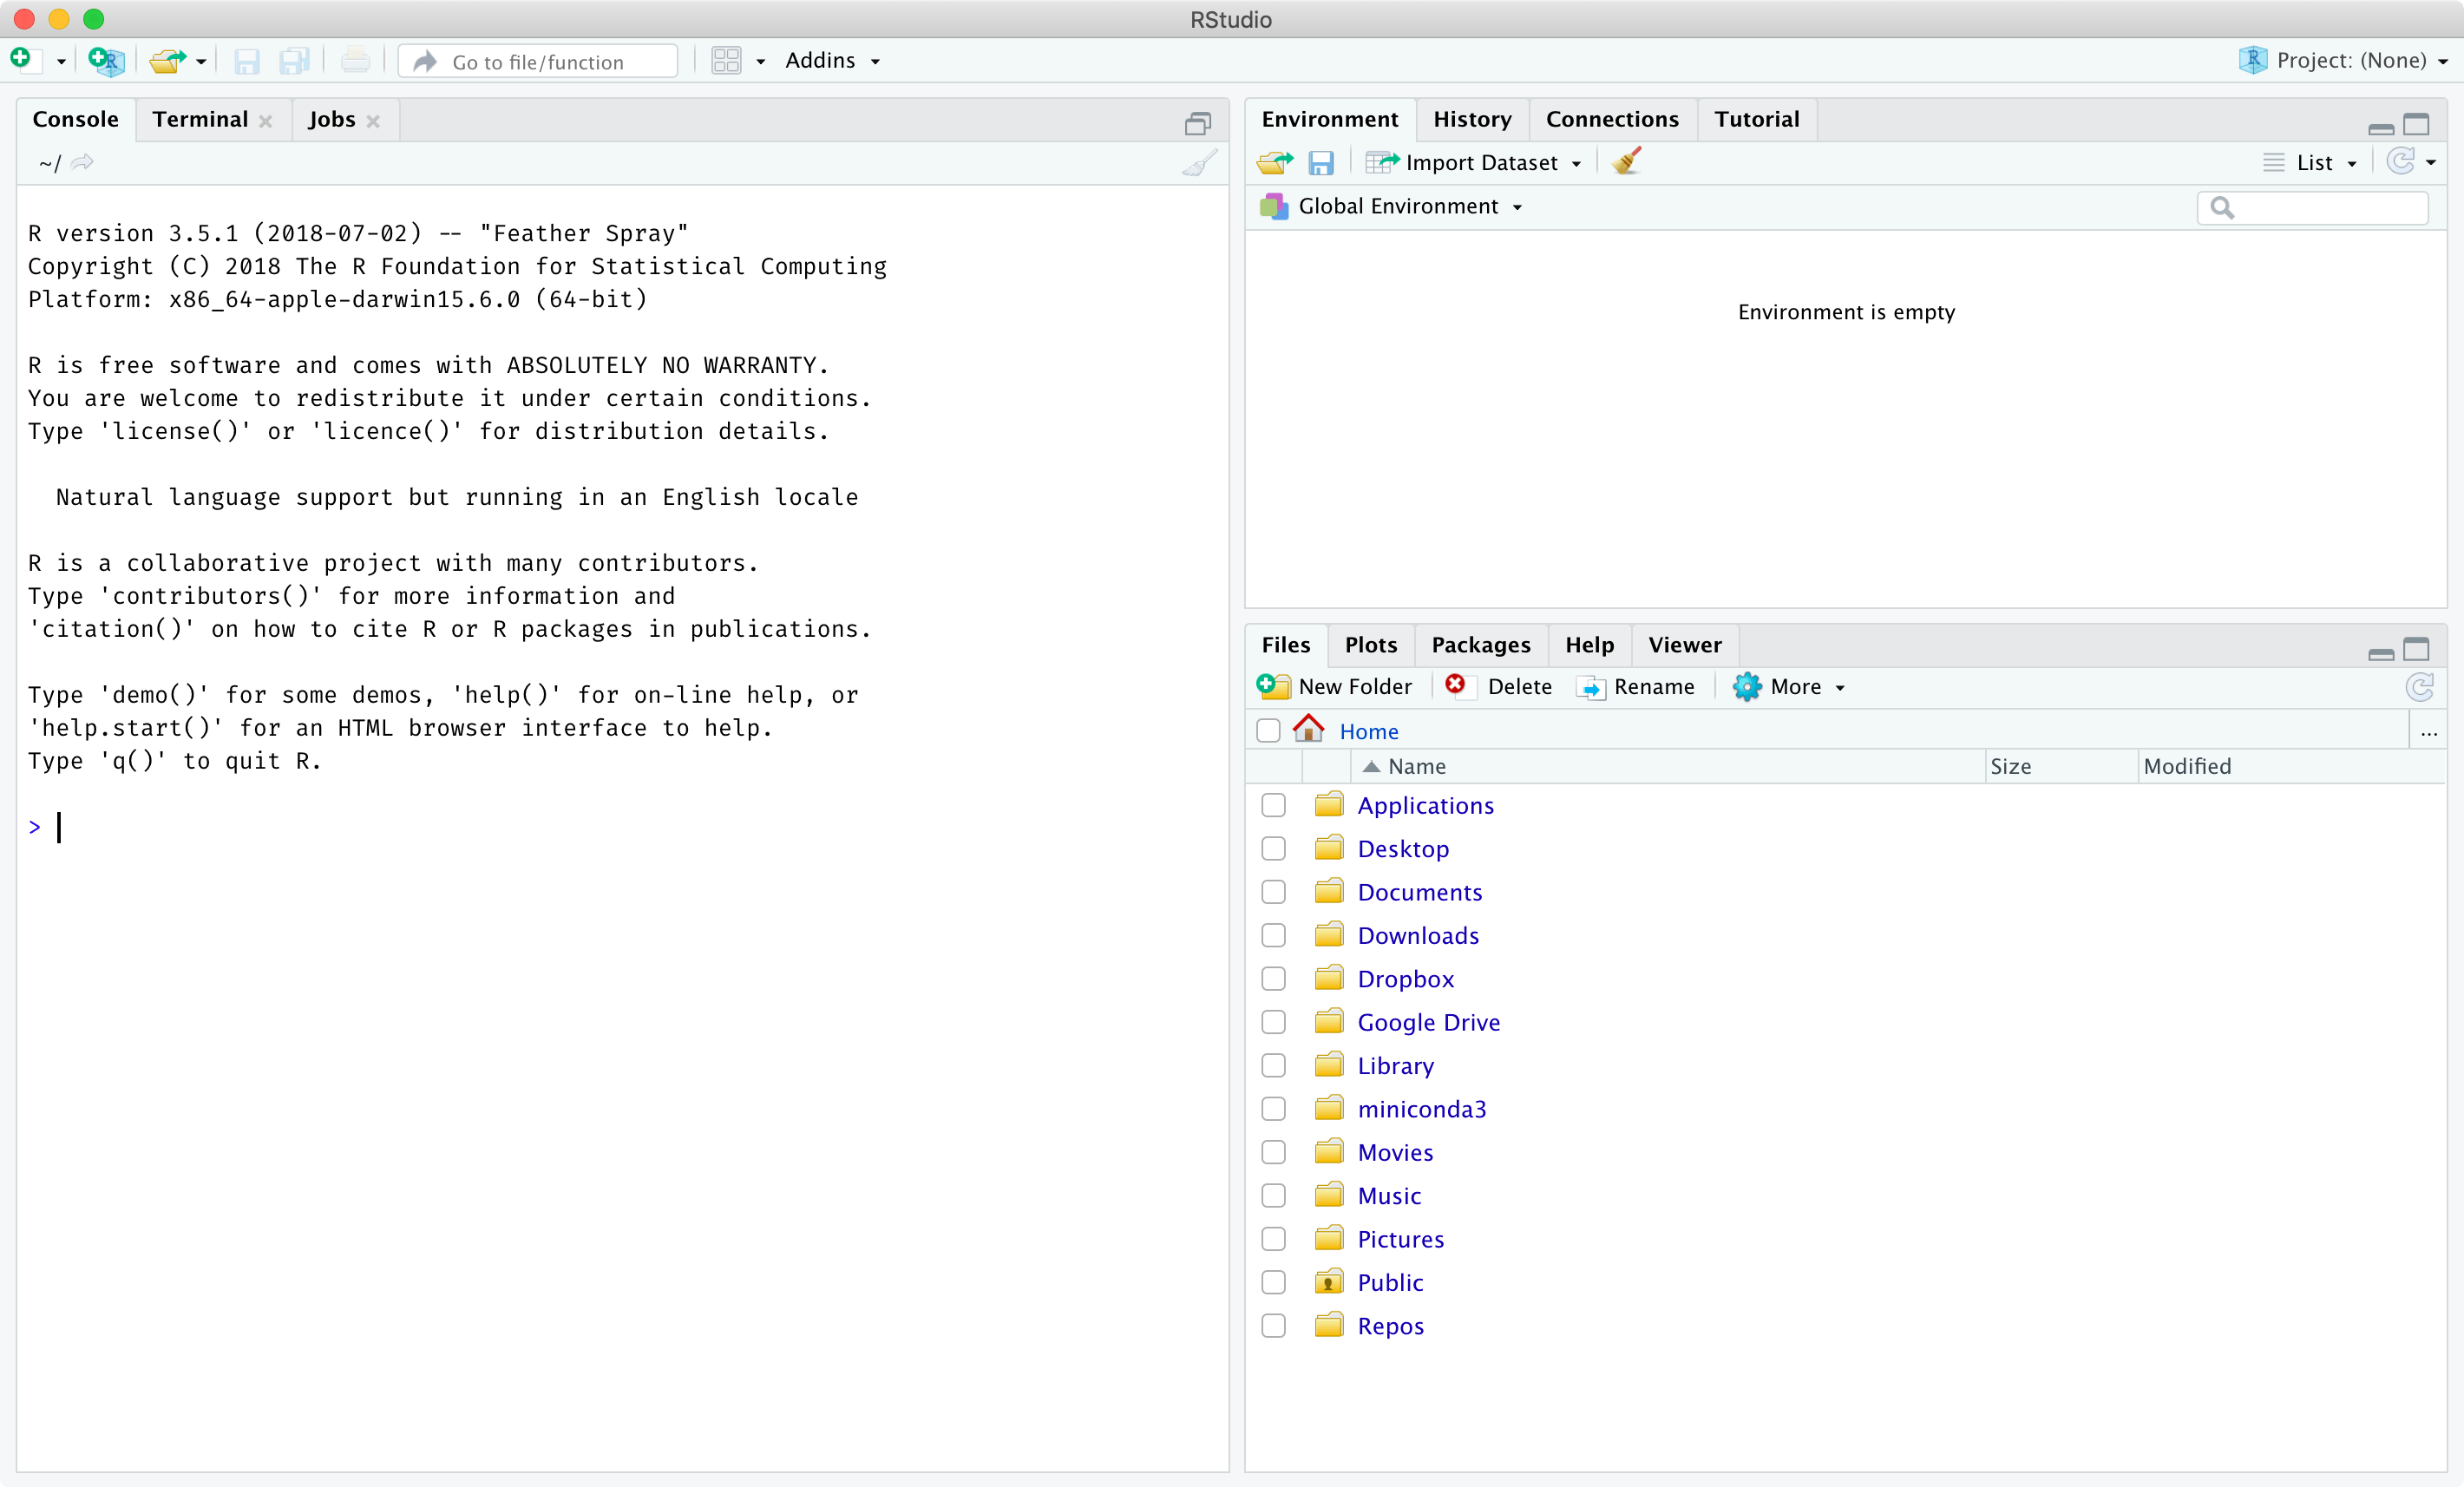
\includegraphics{screenshots/3panes.png}
\caption{Default RStudio Inferface}
\end{figure}

The fourth and final Source pane appears when files are opened
(top-left). Here, a new Untitled R script was created via the top menu
under File \textgreater{} New File \textgreater{} R script. (On macOS,
the top menu is at the top of the screen outside of the RStudio window.)
The Console pane moves to the bottom-left when the Source pane is open.

\begin{figure}
\centering
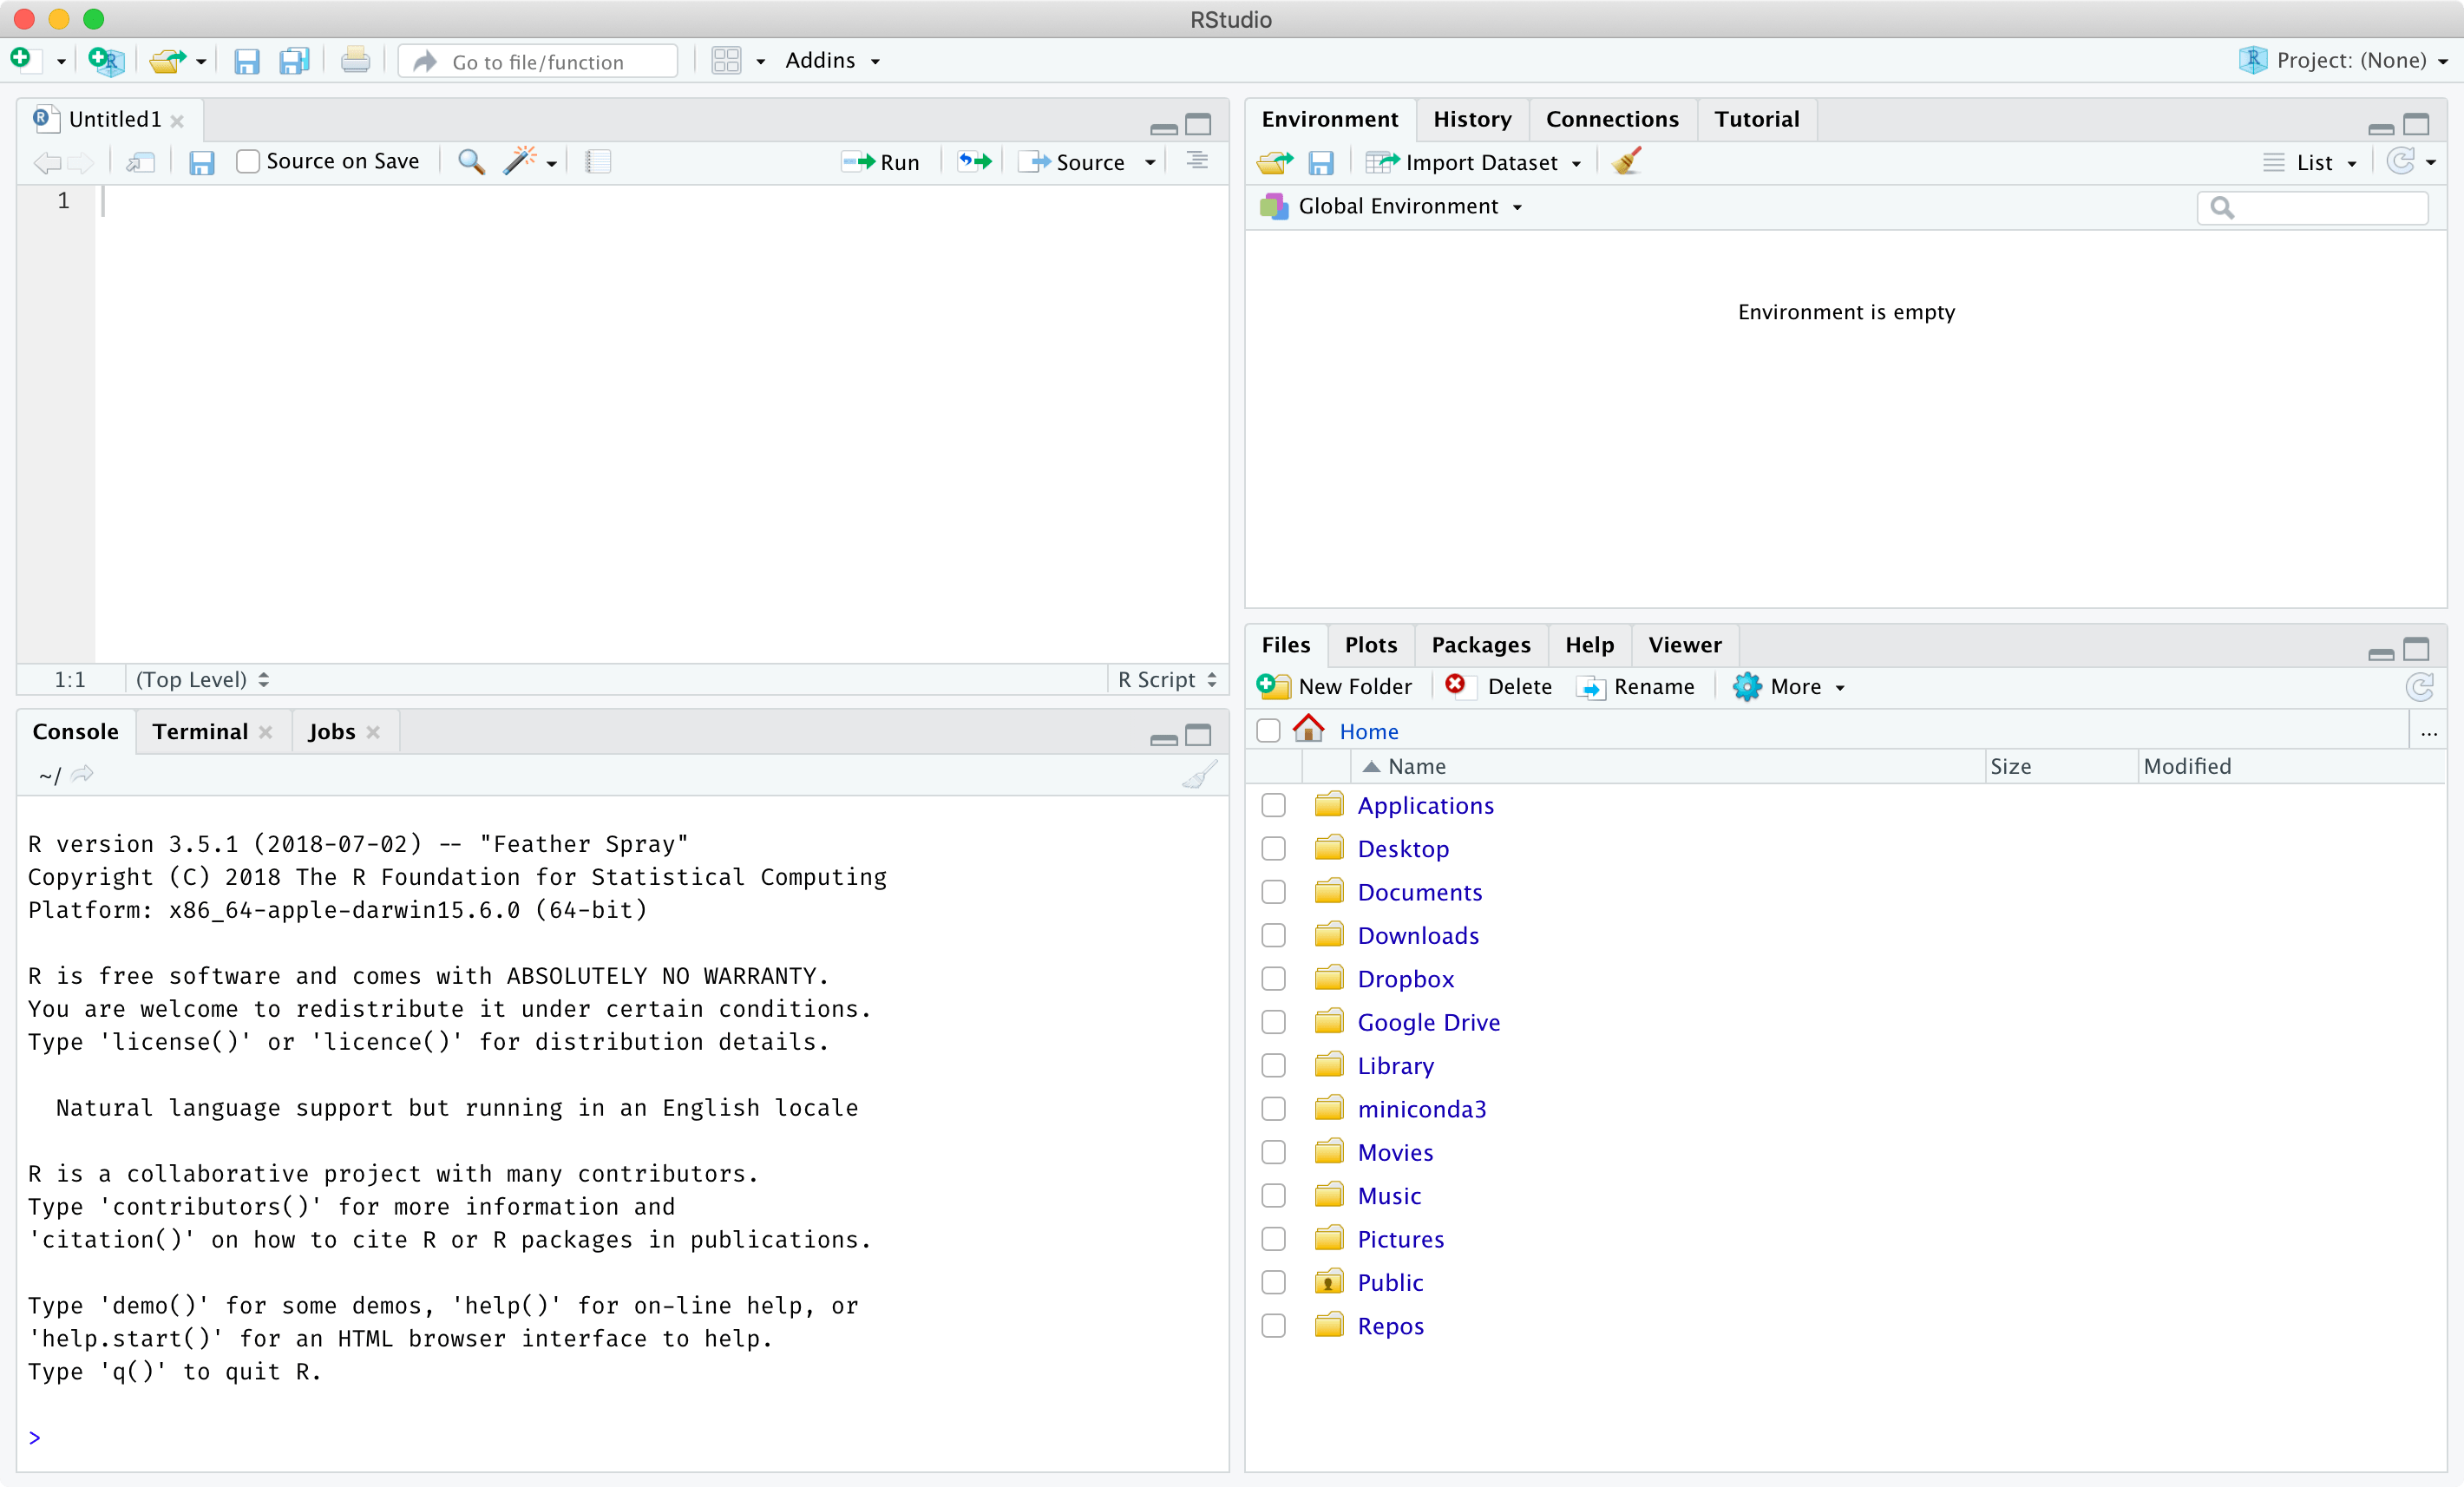
\includegraphics{screenshots/4panes.png}
\caption{New Script in RStudio}
\end{figure}

Before doing anything else, you should update two RStudio settings.
These changes will help ensure that you don't run into any unexpected
behaviour. You can access the RStudio settings via the top menu under
Tools \textgreater{} Global Options. You will want to disable the
following two options, which should appear in the General (Basic tab)
section under Workspace:

\begin{itemize}
\tightlist
\item
  Uncheck ``Restore .RData into workspace at startup''
\item
  Set ``Save workspace to .RData on exit'' to Never
\end{itemize}

The end result should look like this:

\begin{figure}
\centering
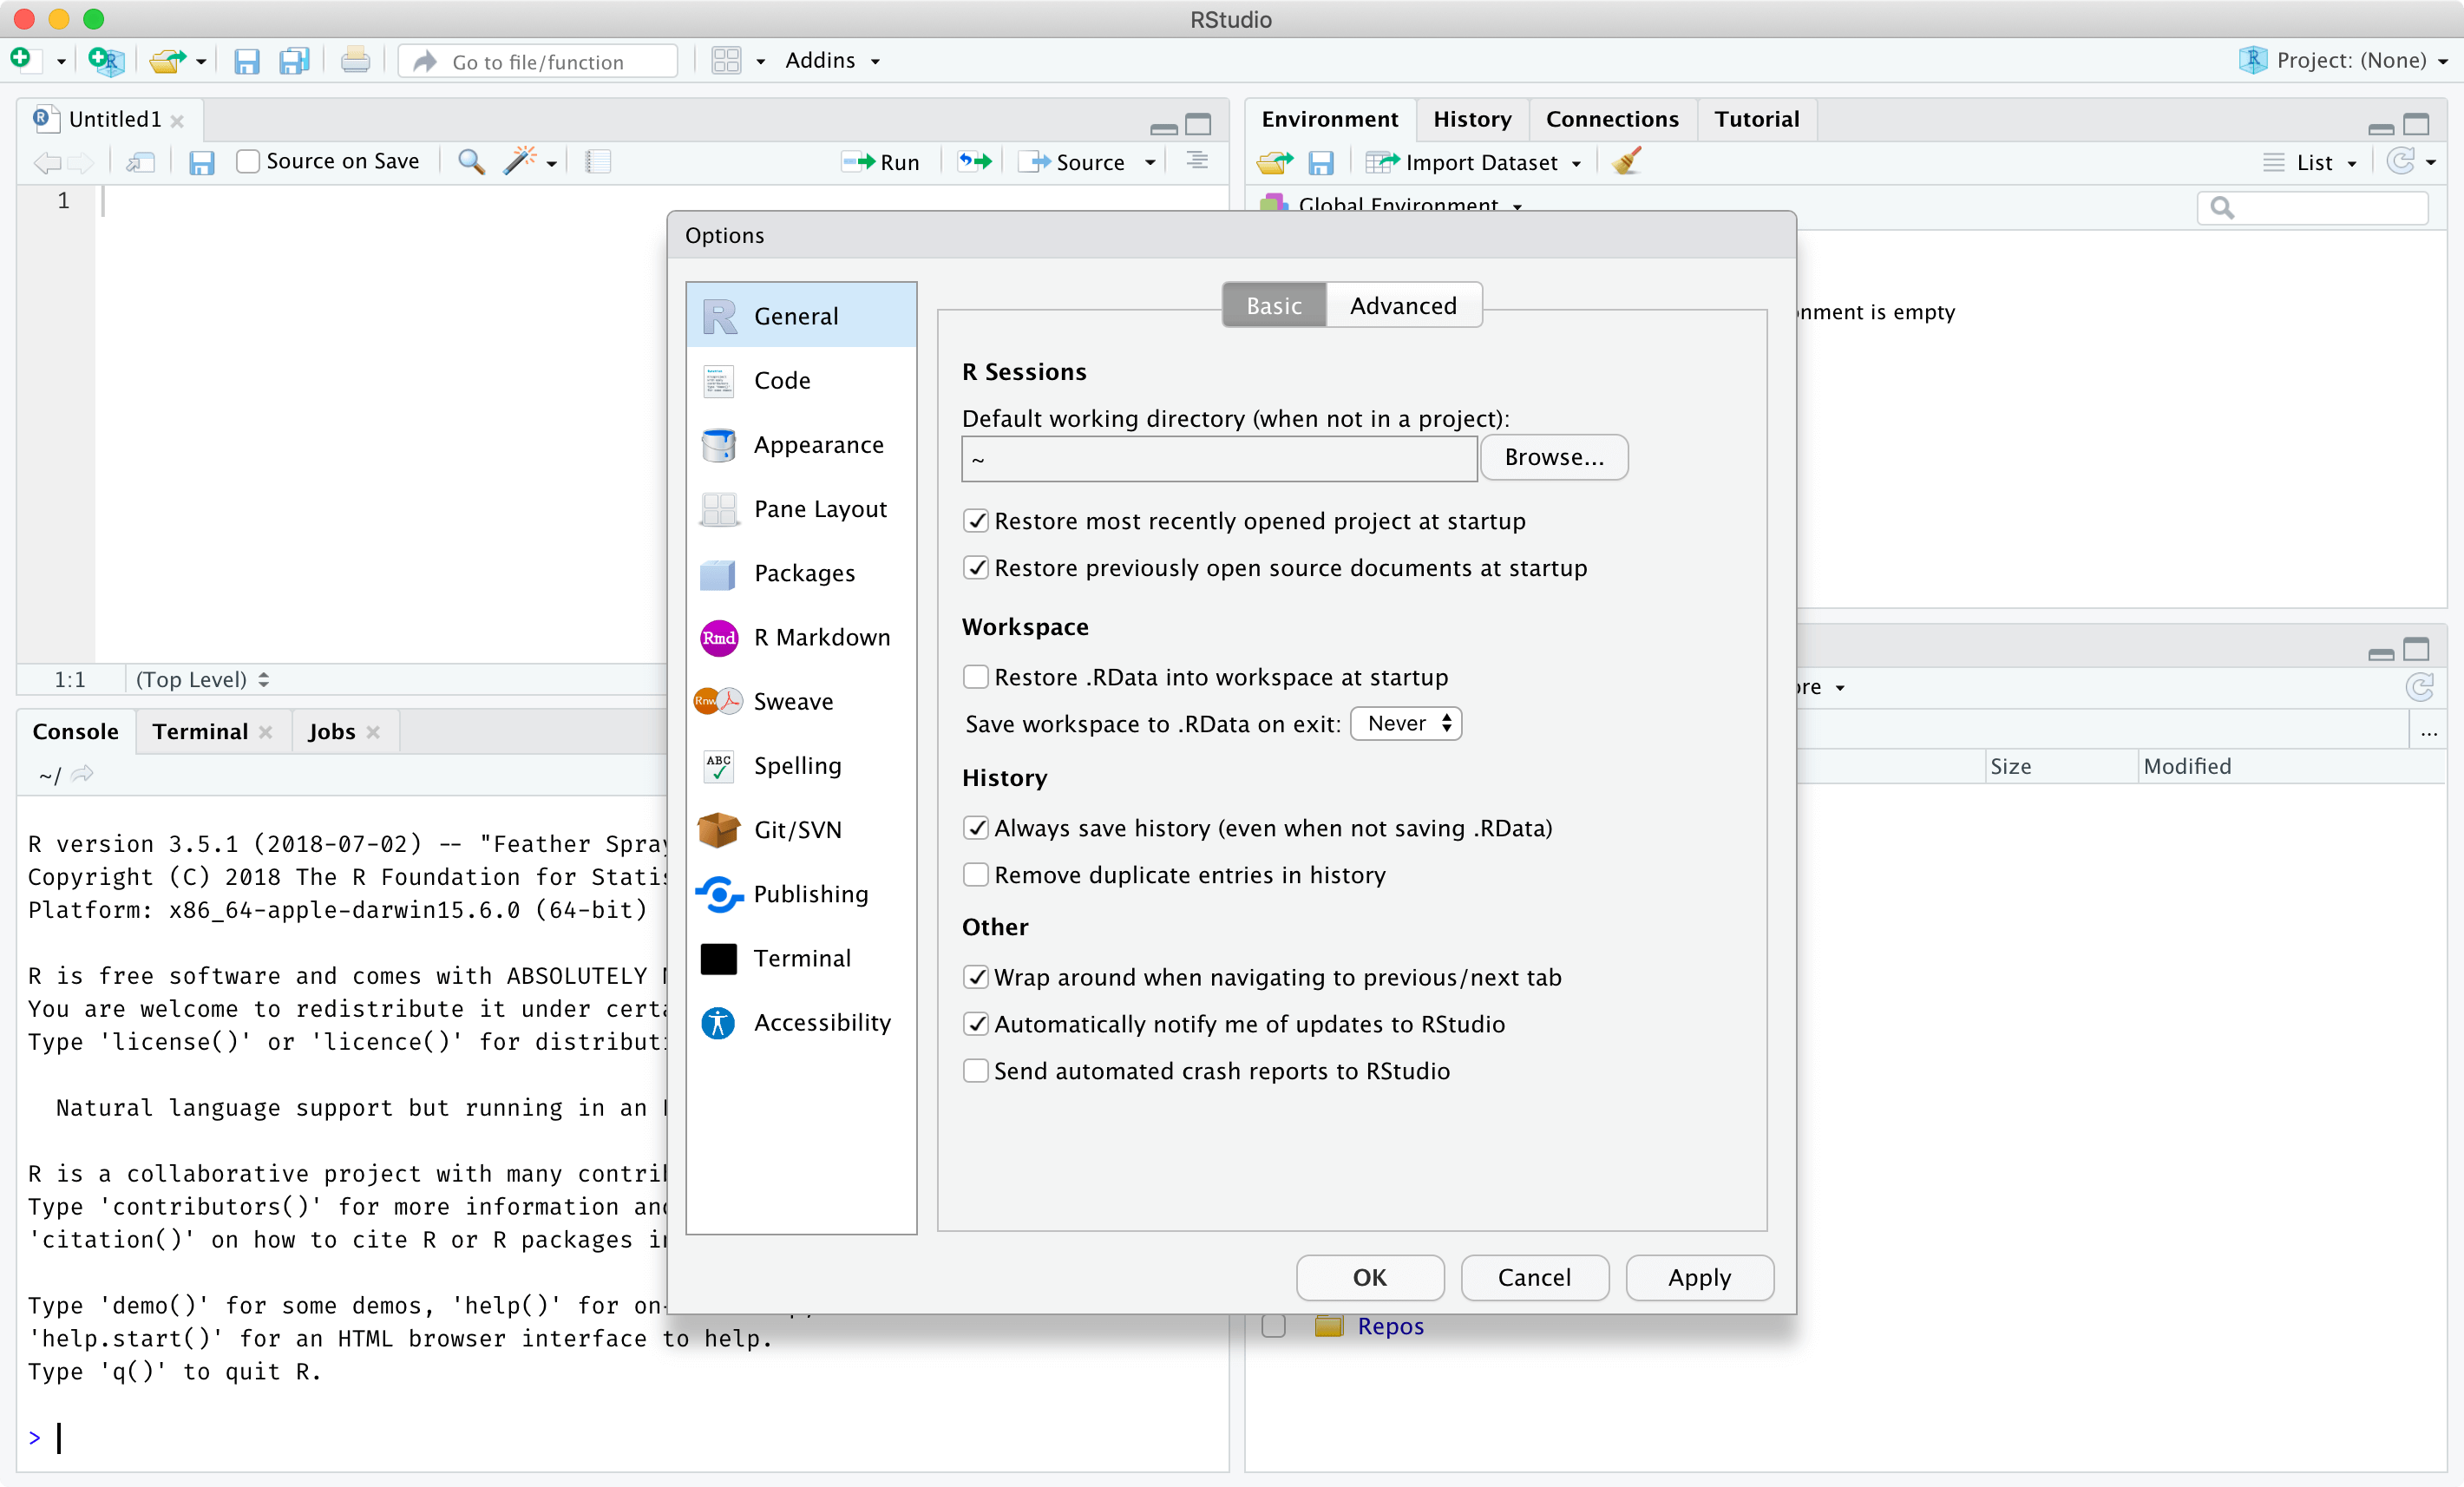
\includegraphics{screenshots/options.png}
\caption{RStudio Global Options}
\end{figure}

There is a wide range of additional options that you can configure in
RStudio based on your personal preference. For example, under the
Appearance section, you can change the zoom level (how big visual
elements like icons appear in RStudio), the font and font size, and the
colour scheme.

\begin{figure}
\centering
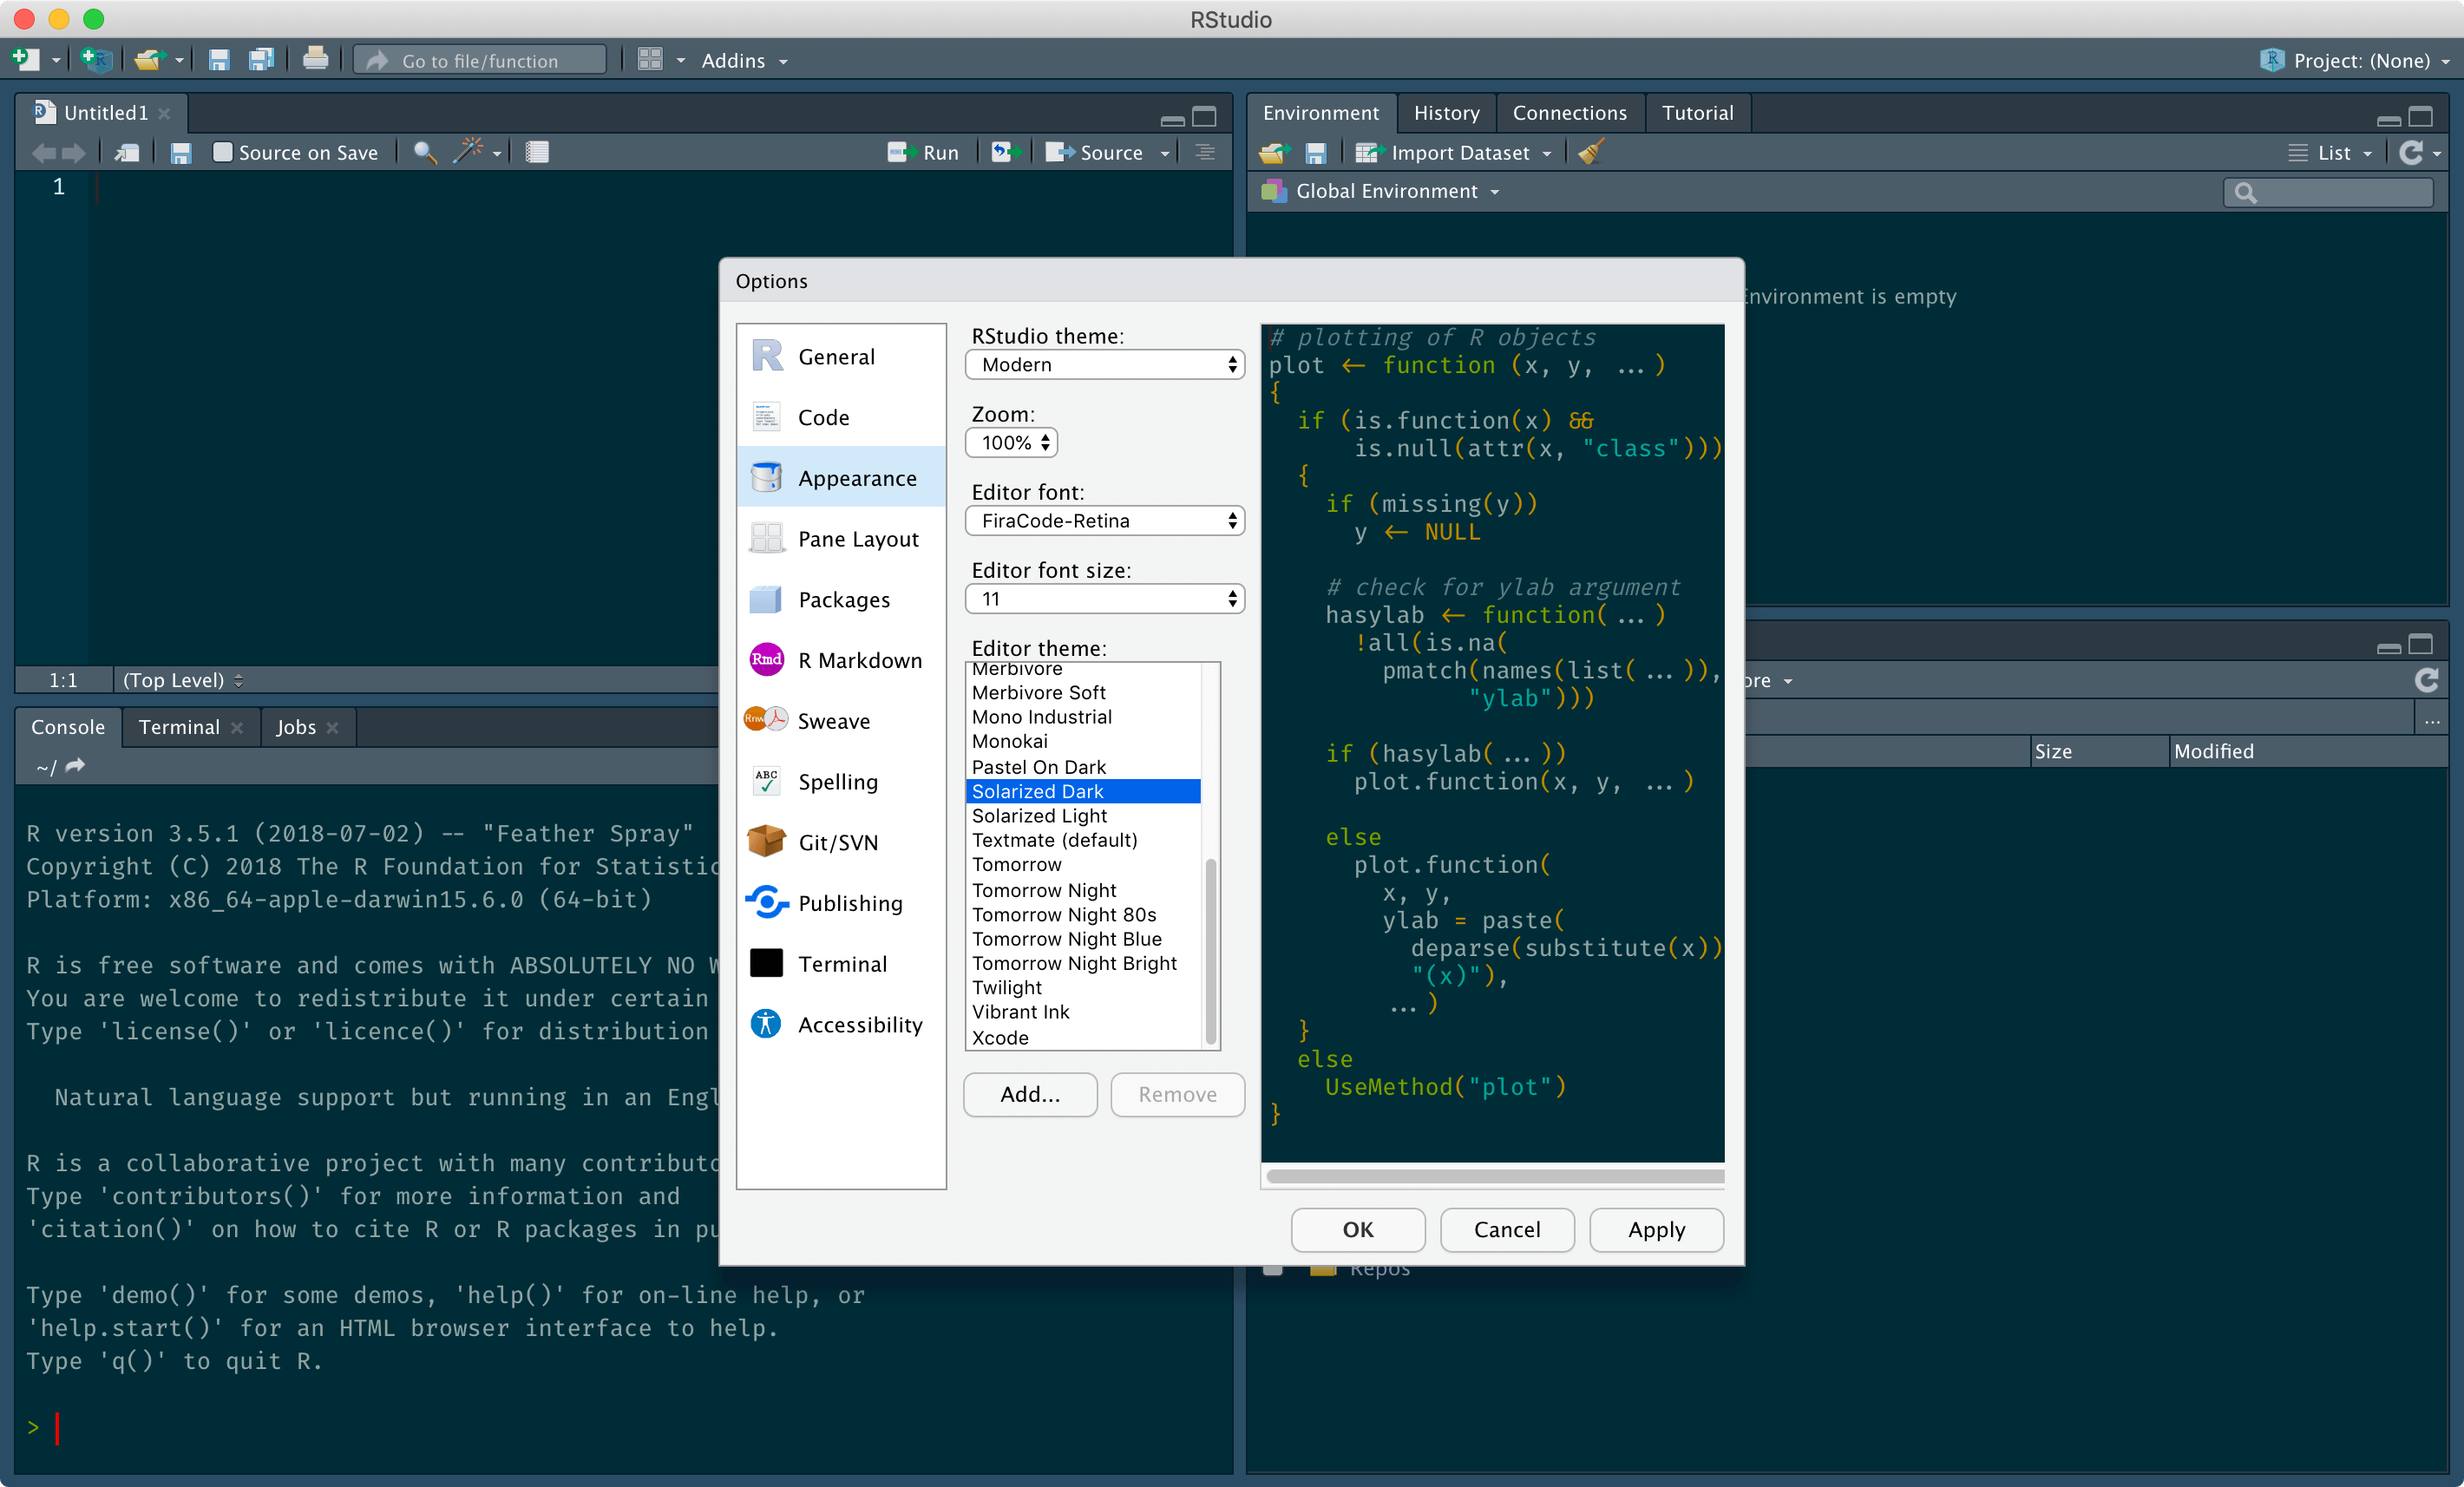
\includegraphics{screenshots/appearance.png}
\caption{RStudio Appearance}
\end{figure}

You can also change the pane locations under the Pane Layout section.
Many RStudio users prefer having their Console pane at the top-right
next to the Source pane because these two panes tend to be the most
important and thus the largest. Again, there is no ``correct'' approach.
Tweak based on what you prefer.

\begin{figure}
\centering
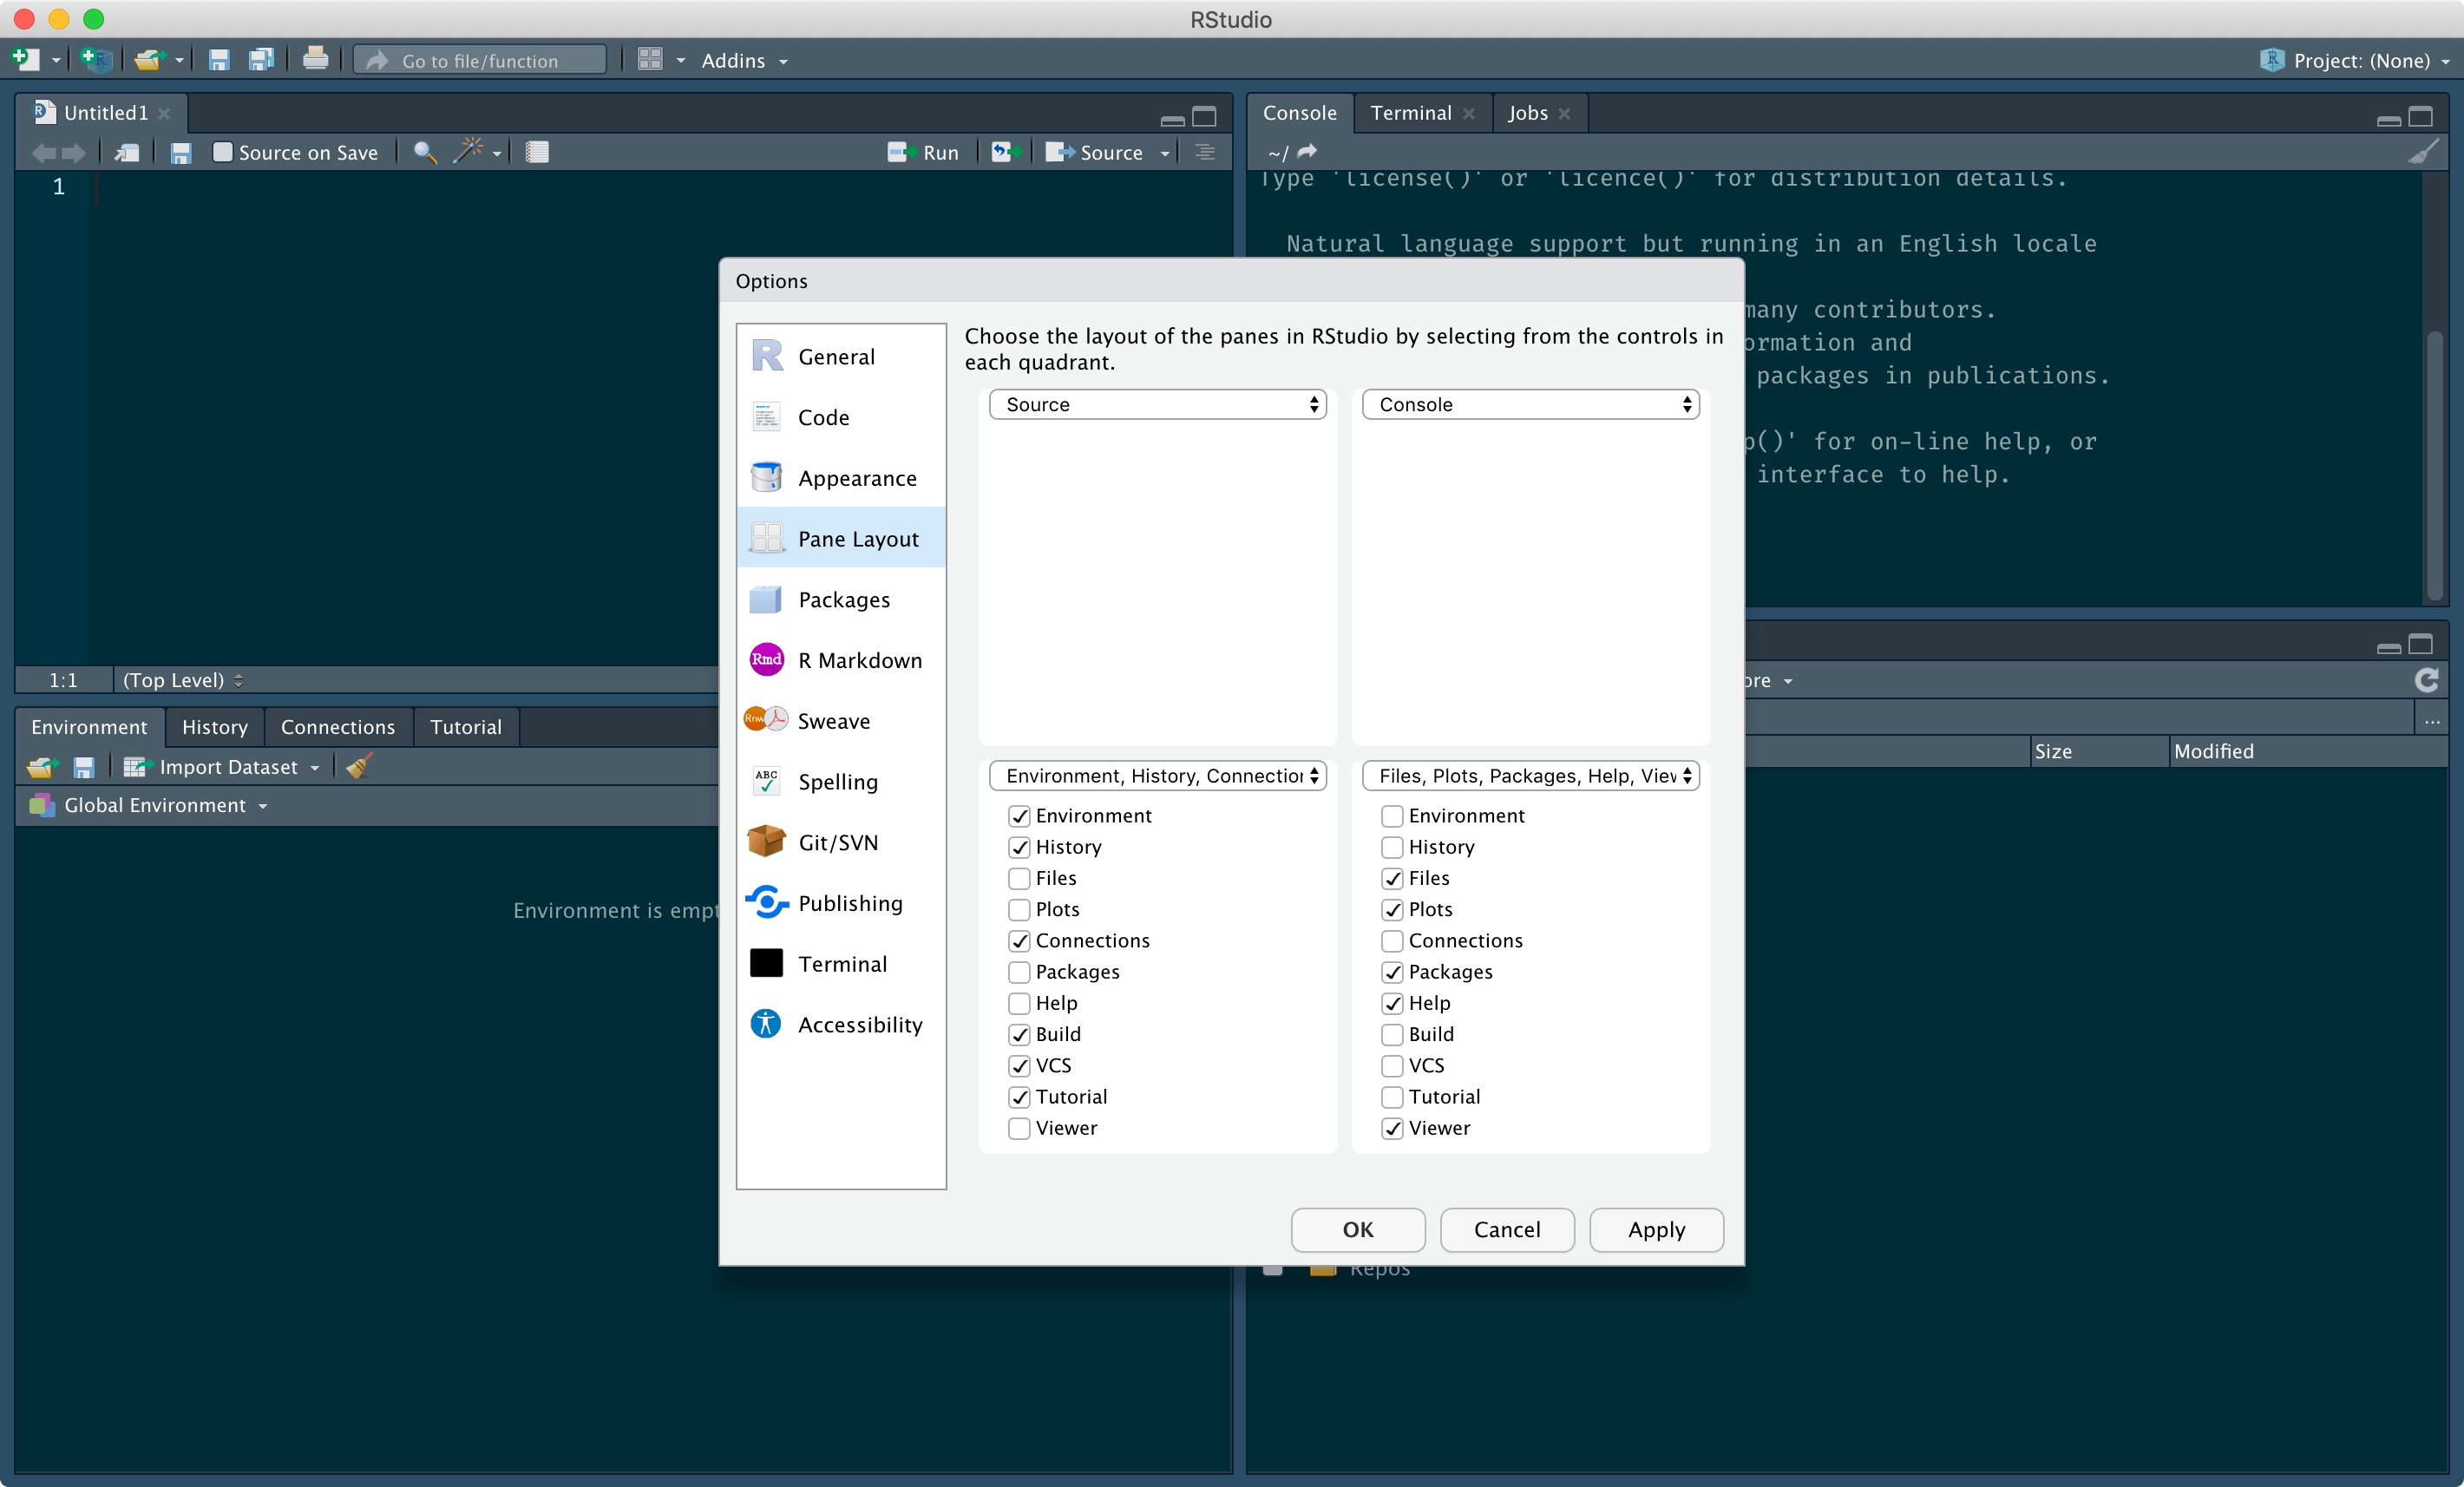
\includegraphics{screenshots/layout.png}
\caption{RStudio Pane Layout}
\end{figure}

Take some time to explore the available settings in the Global Options.
What else did you tweak?

Obviously, another important aspect of RStudio is running R code. There
are two general approaches to running code in RStudio:

\begin{enumerate}
\def\labelenumi{\arabic{enumi}.}
\tightlist
\item
  Run code directly in the Console pane

  \begin{itemize}
  \tightlist
  \item
    This option is convenient for small tasks, but it doesn't scale to
    larger analyses.
  \item
    Relying on the R History for keeping track of past commands is
    tedious and error-prone.
  \end{itemize}
\item
  Write code in the Source pane and selectively run code in the Console

  \begin{itemize}
  \tightlist
  \item
    This is the recommended approach to running R code in RStudio.
  \item
    By storing code in files, you can easily re-run previously used
    code.
  \item
    Button and keyboard shortcuts in RStudio make it easy to run bits of
    code in the console.
  \end{itemize}
\end{enumerate}

When you want to selectively run R code in the Console, you can click
the ``Run'' button at the top-right of the Source pane. If you have code
selected, this will run the selected code. Otherwise, it will run the
line of code where your flashing text cursor is located. If you hover
over the ``Run'' button for a few seconds, you should see an associated
keyboard shortcut. By default, it should be Cmd-Enter on macOS or
Ctrl-Enter on Windows. Commit this to memory, because you will use this
shortcut a lot in this course.

\begin{figure}
\centering
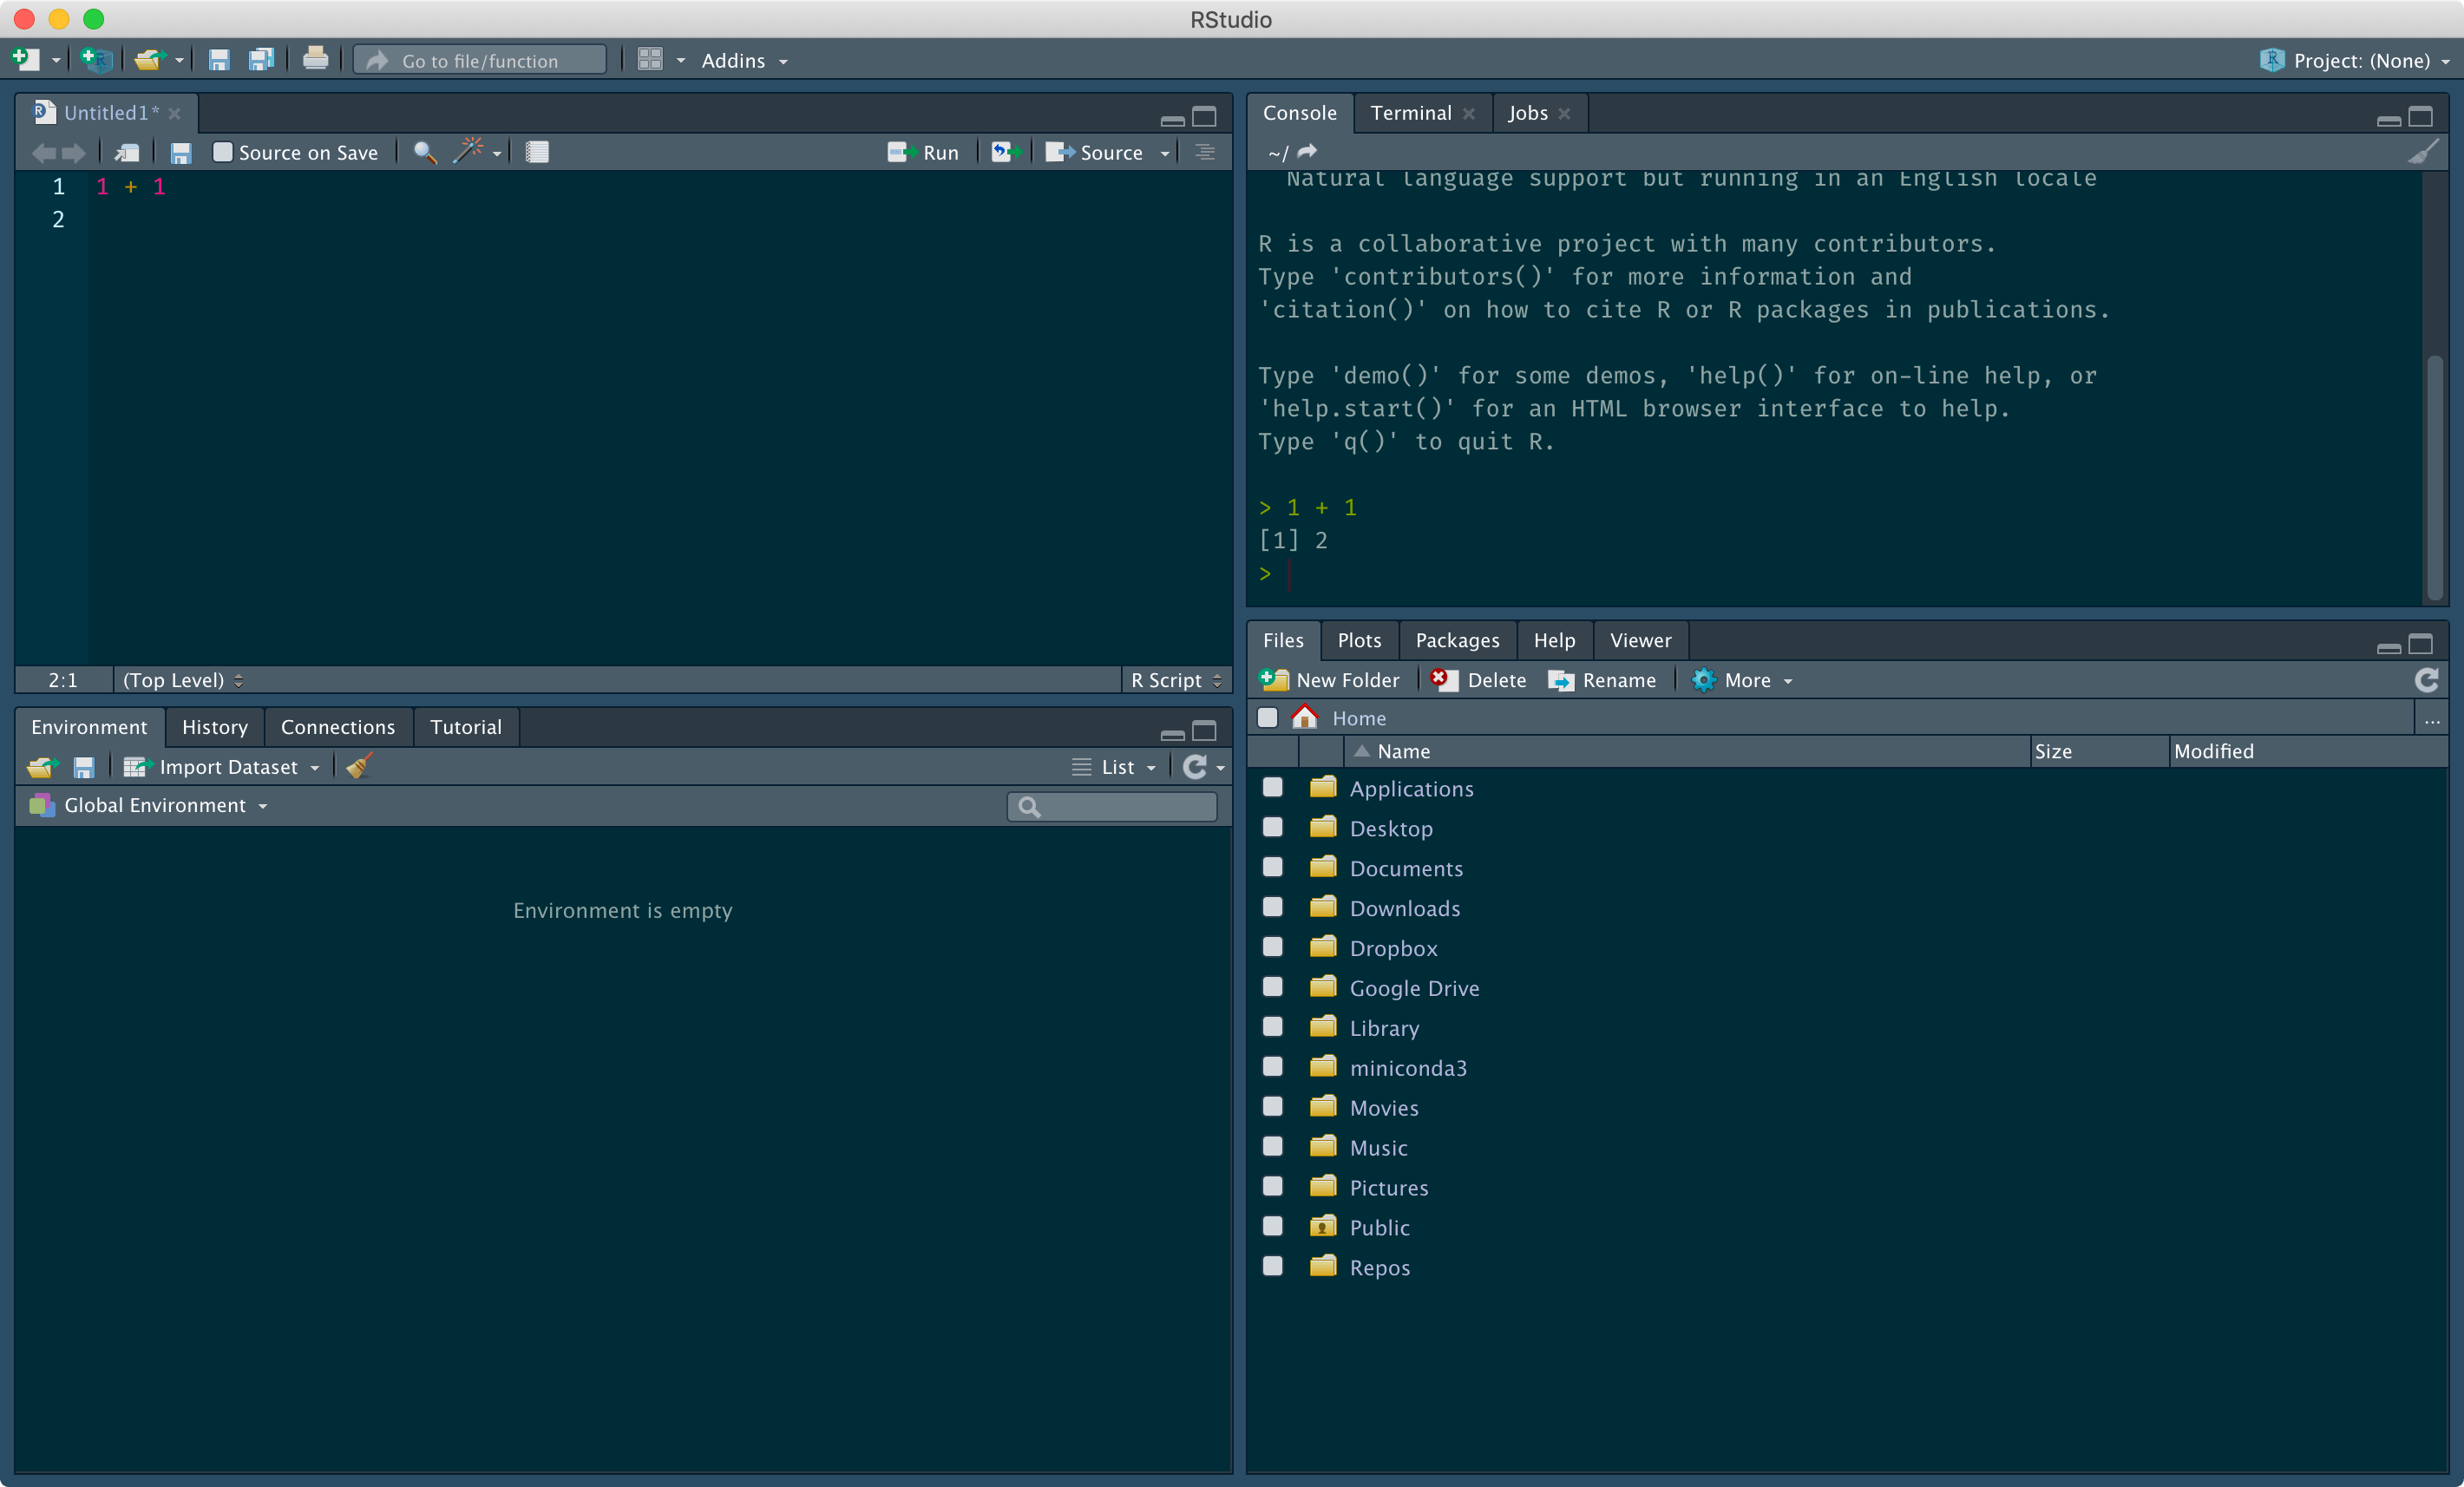
\includegraphics{screenshots/run.png}
\caption{RStudio Source to Console}
\end{figure}

You can open a keyboard shortcut summary via the top menu under Tools
\textgreater{} Keyboard Shortcuts Help. You can also edit keyboard
shortcuts under Tools \textgreater{} Modify Keyboard Shortcuts. These
shortcuts can minimize the time you spend using your mouse/trackpad,
which in turn increases your productivity. It's worthwhile looking up or
setting keyboard shortcuts for anything you do repeatedly.

\begin{figure}
\centering
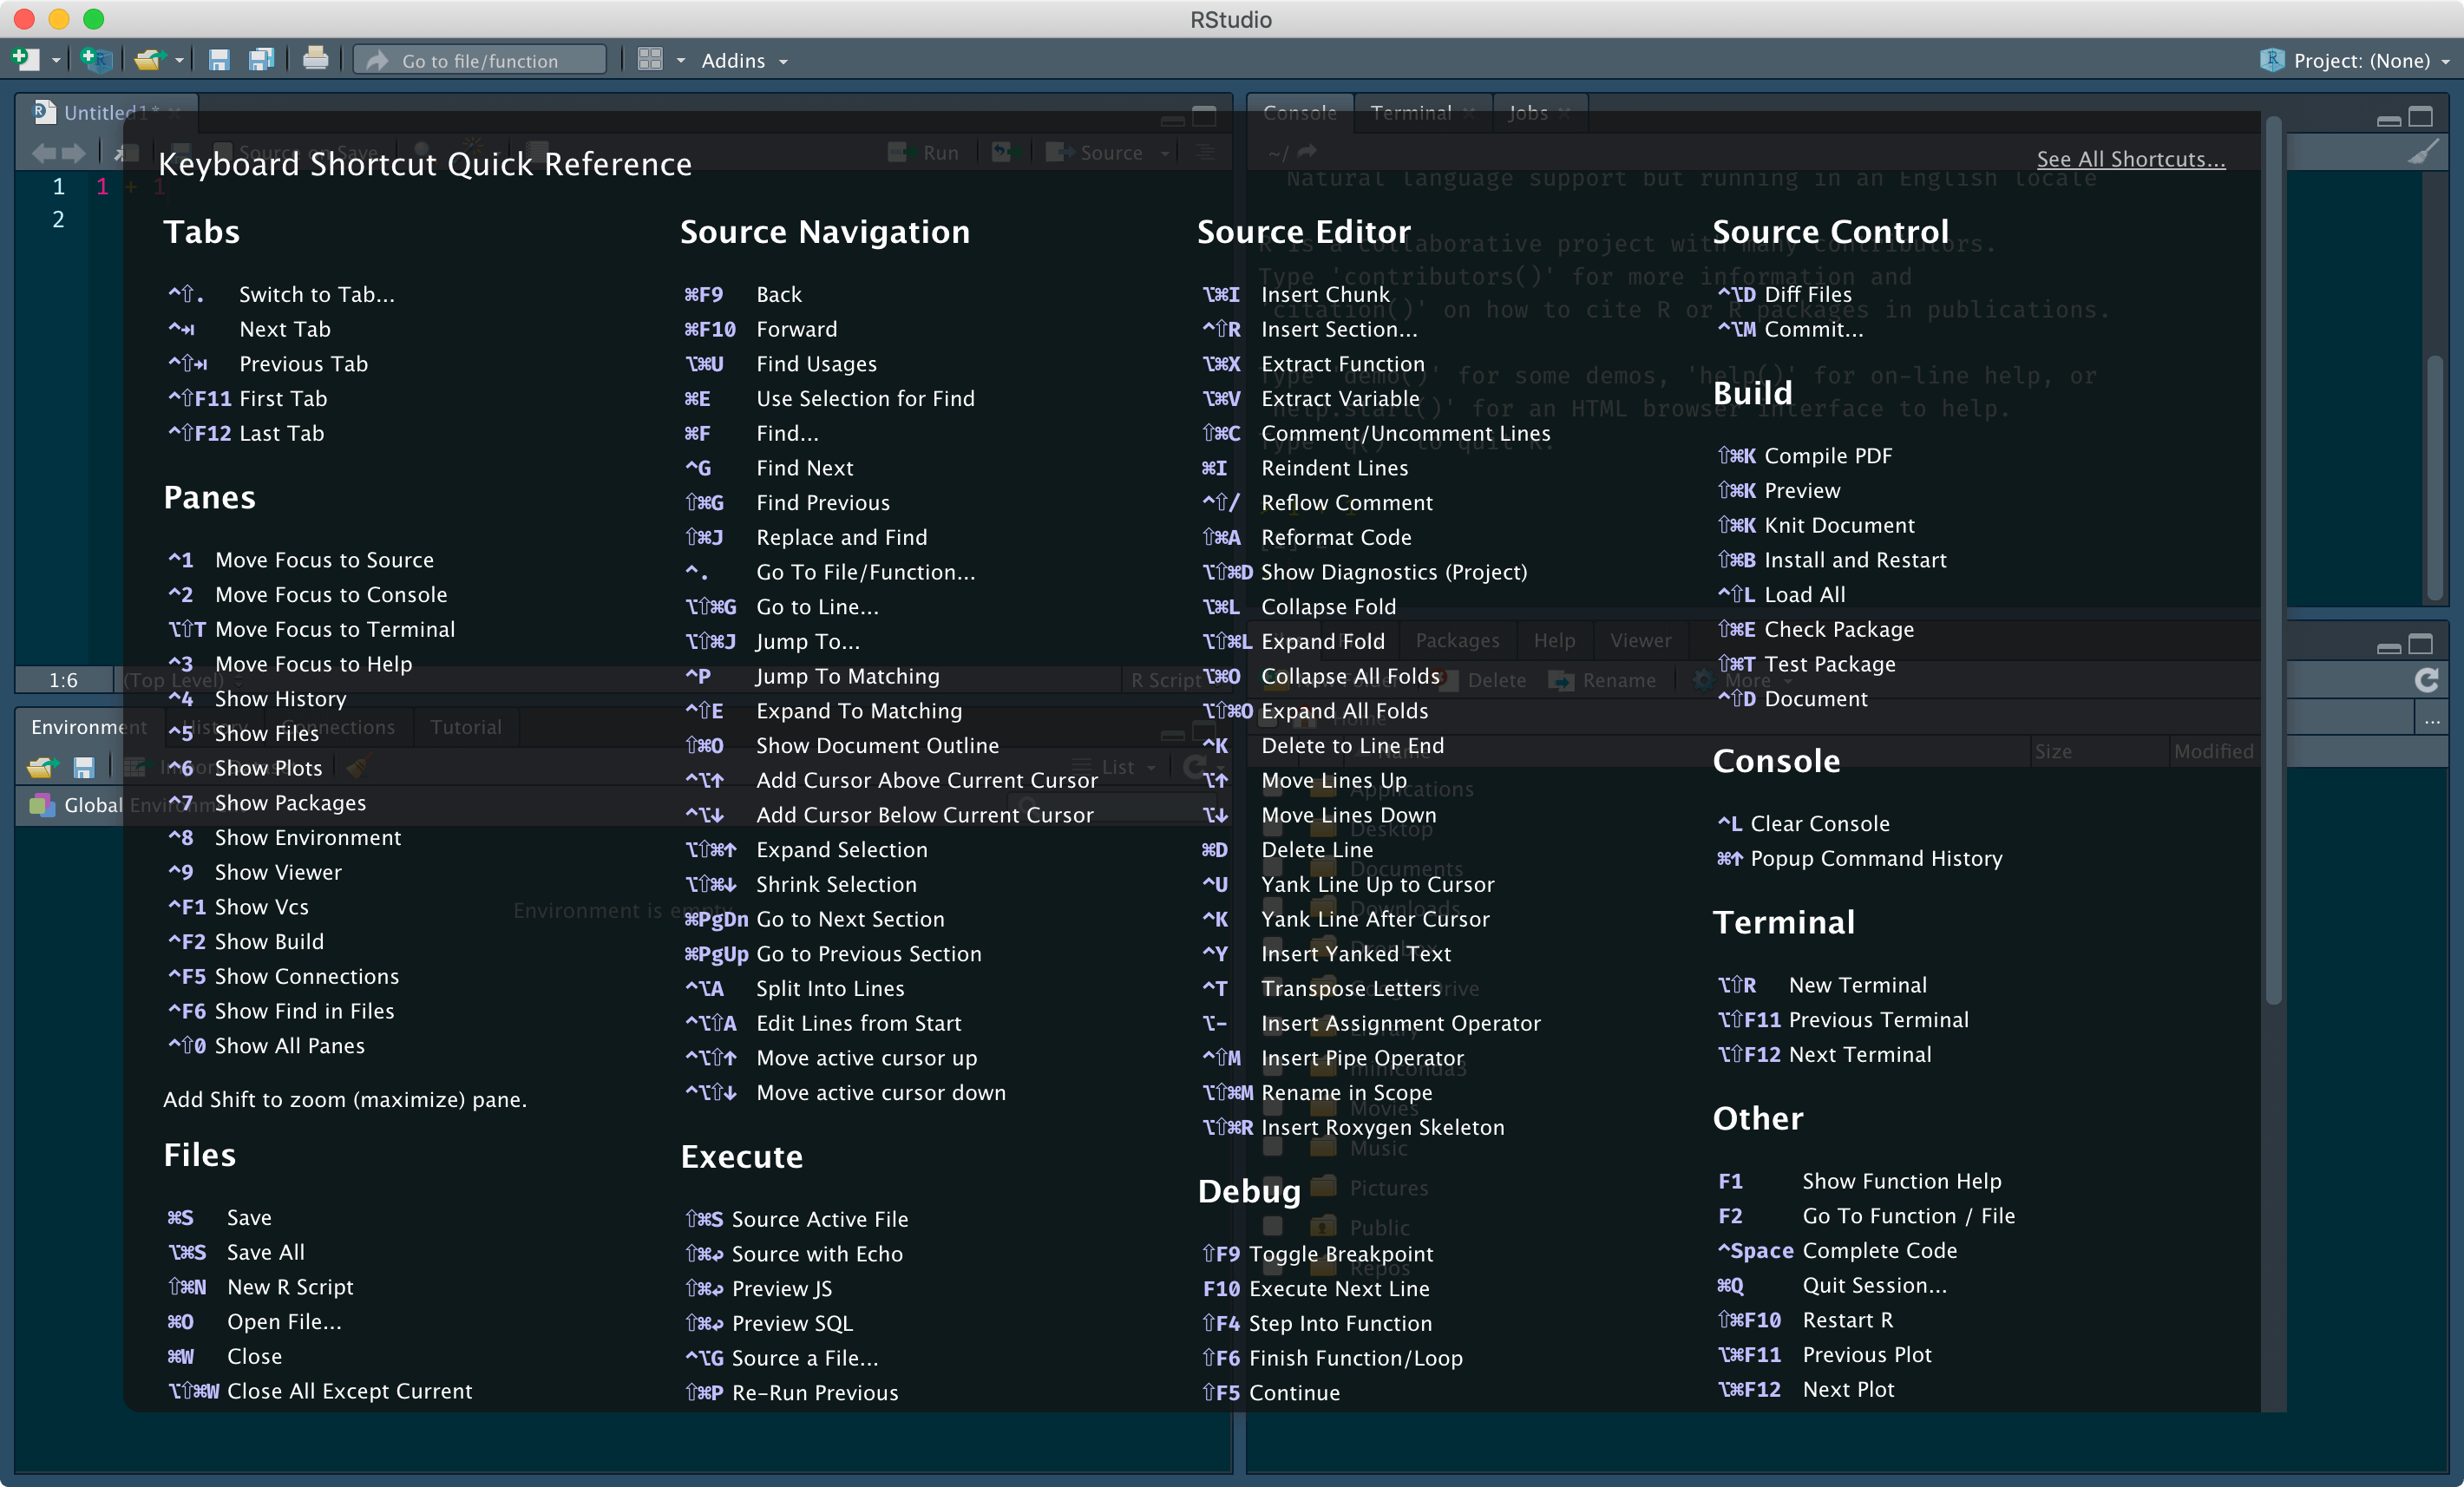
\includegraphics{screenshots/shortcuts.png}
\caption{RStudio Source to Console}
\end{figure}

\hypertarget{syntax-of-these-documents-markdown-and-rmarkdown}{%
\subsection{Syntax of these documents (Markdown and
RMarkdown)}\label{syntax-of-these-documents-markdown-and-rmarkdown}}

All lab materials are derived from
\href{https://rmarkdown.rstudio.com/lesson-1.html}{R Markdown}
documents. These are based on the
\href{https://www.markdownguide.org/getting-started/}{Markdown} syntax,
which in it's purest form is a lightweight markup language for producing
web content with flexible formatting from plaintext documents. but allow
embedded code (with specific formatting) to be used to dynamically
generate content. R Markdown allows the underlying code used for any
analysis to be encapsulated alongside the result (output) of that code.

\hypertarget{r-code-in-rstudio-using-r-markdown}{%
\subsection{R code in RStudio using R
Markdown}\label{r-code-in-rstudio-using-r-markdown}}

As is customary, the first code you see from any programming language is
known as Hello World and is somewhat self-explanatory. If you look
immediately below this text in the Rmd file you will see three lines.
The first line has three ``backtick'' characters, i.e.~these:

\textbf{`}

The backtick is found to the left of the 1 key and is not to be confused
with a single quotation mark. In R Markdown, anything surrounded by
either a pair of backticks or two triplets of backticks is considered
code that should be executed.

\begin{Shaded}
\begin{Highlighting}[]
\NormalTok{to\_print }\OtherTok{\textless{}{-}} \StringTok{"Hello World"}
\CommentTok{\#this is a comment and will be ignored by the compiler}
\FunctionTok{print}\NormalTok{(to\_print)  }\CommentTok{\# everything to the right of any \# will also be ignored but the code to the left of it is not ignored}
\end{Highlighting}
\end{Shaded}

\begin{verbatim}
## [1] "Hello World"
\end{verbatim}

\begin{Shaded}
\begin{Highlighting}[]
\CommentTok{\# print(nonexistent\_variable)}
\CommentTok{\# The line above is code that has been converted to a comment. This is what is typically referred to as "commented out". You may encounter code in this form that you will need to "uncomment" by deleting the first \#. If you do that to the comment line above, what happens?}
\end{Highlighting}
\end{Shaded}

Most of the code you will see in labs will be in the format above.
Inline R code is less readable but allows the output of R to be inserted
directly into paragraphs such as this Hello World example, which re-uses
the variable we created above. In the next lab you will learn more about
variables and their uses.

\hypertarget{what-to-do-when-you-get-stuck}{%
\subsection{What to do when you get
stuck}\label{what-to-do-when-you-get-stuck}}

One of the most important skills in programming (and life maybe?) is
framing a question with sufficient context and detail such that others
can answer it. The basic Markdown syntax we use here is available in
Slack, GitHub, StackOverflow (to name a few) and many other web-based
resources for programmers. Below are two examples of questions with the
first a ``bad'' example, which is unlikely to be answer-able and the
second a ``good'' example. This is all using pure Markdown without any
code meant for interpretation by R.

\hypertarget{example-question-1}{%
\subsubsection{Example Question 1}\label{example-question-1}}

\textbf{Posting Title: R is broken}

I'm getting this error message from R and I don't know what it means.
Can u plz help my assignment is due tomorrow!?!

Error: unexpected symbol in ``print hello''

\hypertarget{example-question-2}{%
\subsubsection{Example Question 2}\label{example-question-2}}

\textbf{Posting Title: Issue with printing a variable in R}

When I run the following R code I keep getting the error message shown
below. I'm attempting to reproduce a simple example from a class. My
intention is to set the variable \texttt{hello} with the character
string ``hello world'' and then print that variable to the screen. I get
the same result in a fresh/new R session. Can someone please help me
find the error?

\begin{verbatim}
hello <- "hello world"
print hello
\end{verbatim}

\begin{quote}
Error: unexpected symbol in ``print hello''
\end{quote}

\textbf{Task}

At some point during the semester, every student must post at least one
good question to the course StackOverflow page. Ideally this will happen
naturally when each of you inevitably get stuck. If you don't get stuck
you can still mock up a question and post it. \emph{This will be counted
towards the participation component of your mark.}

\hypertarget{more-resources}{%
\subsection{More Resources}\label{more-resources}}

\begin{itemize}
\tightlist
\item
  \url{https://wordpress.com/support/markdown-quick-reference/}
\item
  \url{http://swcarpentry.github.io/r-novice-gapminder/01-rstudio-intro}
\item
  \url{http://swcarpentry.github.io/r-novice-gapminder/03-seeking-help}
\item
  \url{https://ariel.rbind.io/workshop/rbasics/\#interactive-tutorials}
\end{itemize}

\end{document}
